
%We begin by creating the main page of the client
\begin{figure}[H]

	\centering 
	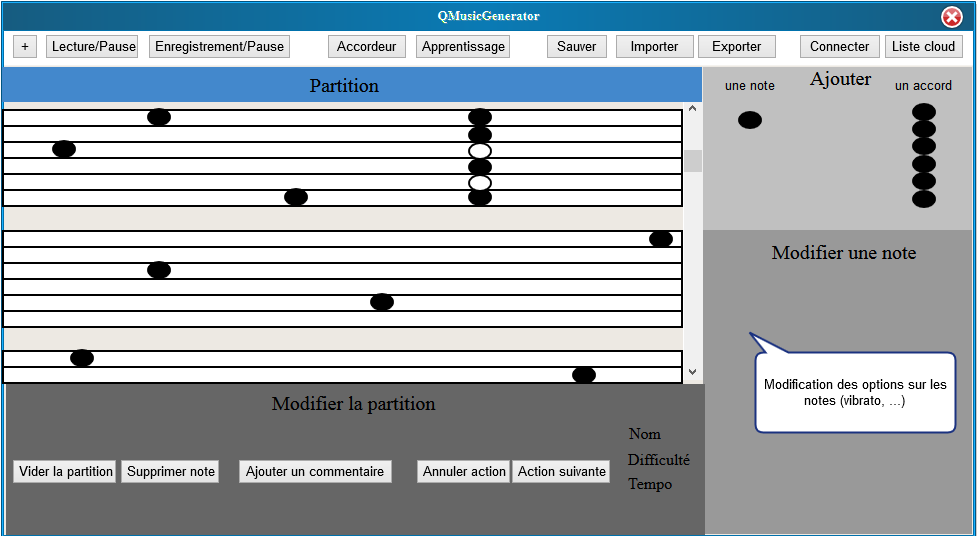
\includegraphics[scale=0.4]{main_page}
		\caption{Page principale du client}
			Cette fenêtre est la fenêtre principale de notre client. A partir de celui-ci, il sera possible
			de créer des partitions vierges, d'en ouvrir des préexistantes, d'en lire et d'enregistrer des 
			notes à partir de l'entrée audio ainsi que de les sauvegarder. \\
			Mais il sera aussi possible d'ouvrir un accordeur, de télécharger des partitions hébergées sur le
			site web, et d'en uploader. \\
			Il sera en effet possible de connecter directement le client avec le site à l'aide des 
			identifiants de l'utilisateur. \\
			De plus, il y aura aussi évidemment toutes les options permettant de modifier la partition en 
			cours, tels que son nom, sa difficulté, son tempo, ... \\
			Enfin, on pourra modifier la partition manuellement en déplaçant les notes ou en en ajoutant. 

\end{figure}

%Then the options list
\begin{figure}[H]

	\centering 
	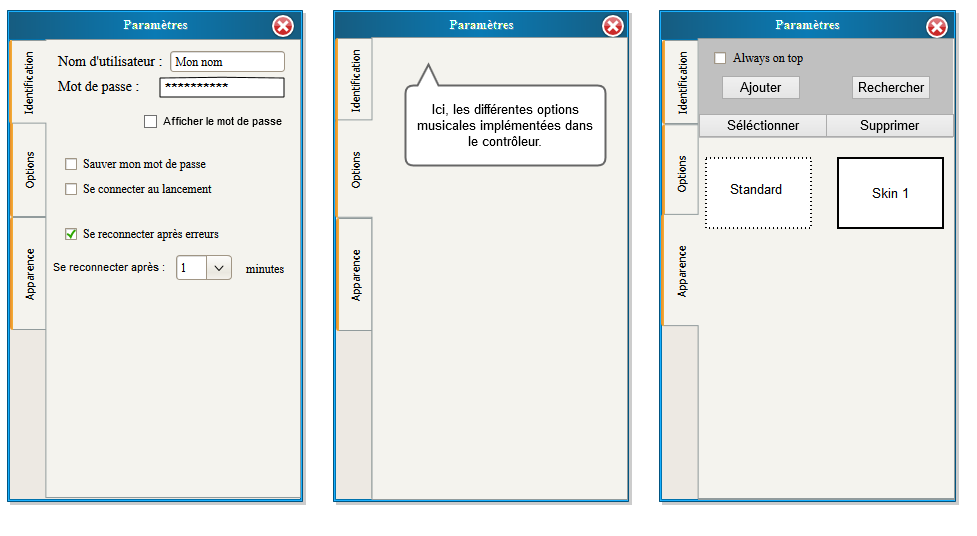
\includegraphics[scale=0.4]{parameters}
		\caption{Fenêtre des paramètres du logiciel}
			Cette fenêtre permettra de modifier les paramètres du logiciel. \\
			Cela recouvre les paramètres d'authentification, ceux spécifiques à la synthèse de musique en
			elle-même, mais aussi l'apparence du client via l'utilisation de skins.

\end{figure}

%And the tablatures list
\begin{figure}[H]

	\centering 
	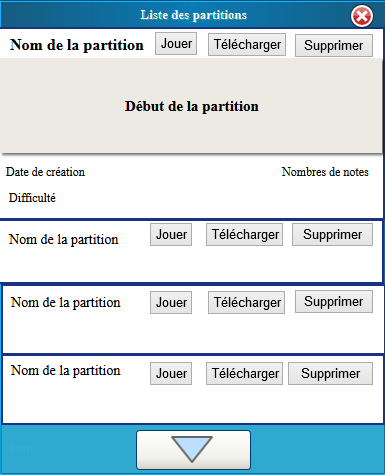
\includegraphics[scale=0.6]{tab_list}
		\caption{Fenêtre des listes de partitions hébergées sur le site web}
			Cette fenêtre listera toutes les partitions que l'utilisateur a uploadé sur le site internet si 
			celui-ci est connecté. \\
			A partir de cette fenêtre, il pourra soit les supprimer du site web, soit les télcharger, ou 
			encore les jouer.
\end{figure}
%Finally, we put the chord
\begin{figure}[H]

	\centering 
	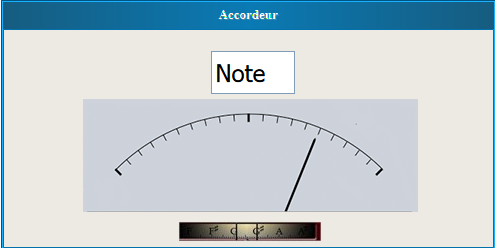
\includegraphics[scale=0.8]{chord}
		\caption{Accordeur}
			Cette fenêtre affichera un accordeur qui analysera l'entrée sonore pour permettre à l'utilisateur
			de réaccorder son instrument directement depuis le logiciel.

\end{figure}
